% ============================================================
%  Segment Tree - CSE200 Presentation
%  PART I -- INTRODUCTION & MOTIVATION (Shuvo)
% ============================================================
\documentclass[10pt,aspectratio=169]{beamer}

\usepackage[T1]{fontenc}
\usepackage{lmodern}
\usepackage{amsmath, amssymb}
\usepackage{booktabs}
\usepackage{colortbl}
\usepackage[normalem]{ulem}
\usepackage{pifont}
\usepackage{tikz}
\usepackage{pgfplots}
\pgfplotsset{compat=1.18}
\usetikzlibrary{decorations.pathreplacing, positioning, calc, arrows.meta}

\usetheme{default}
\useinnertheme{rectangles}
\setbeamertemplate{navigation symbols}{}

% ---------- Color palette (same as master deck) ----------
\definecolor{navy}{RGB}{25,45,90}
\definecolor{deepblue}{RGB}{40,80,150}
\definecolor{lightblue}{RGB}{200,220,240}
\definecolor{cream}{RGB}{252,246,225}
\definecolor{gold}{RGB}{200,155,55}
\definecolor{darkgold}{RGB}{160,120,40}
\definecolor{accentgreen}{RGB}{45,140,80}
\colorlet{softgreen}{accentgreen!15}
\definecolor{warningred}{RGB}{180,50,50}

\setbeamercolor{title}{fg=navy}
\setbeamercolor{subtitle}{fg=deepblue}
\setbeamercolor{frametitle}{fg=white, bg=navy}
\setbeamercolor{frametitle rule}{bg=gold}
\setbeamercolor{structure}{fg=deepblue}
\setbeamercolor{block title}{bg=navy, fg=white}
\setbeamercolor{block body}{bg=lightblue!30, fg=black!85}

\setbeamerfont{frametitle}{series=\bfseries, size=\large}

\setbeamertemplate{frametitle}{%
  \nointerlineskip%
  \begin{beamercolorbox}[wd=\paperwidth, ht=3.0ex, dp=1.2ex, leftskip=0.5cm, rightskip=0.5cm]{frametitle}%
    \usebeamerfont{frametitle}\insertframetitle%
  \end{beamercolorbox}%
  \nointerlineskip%
  \begin{beamercolorbox}[wd=\paperwidth, ht=1.1pt, dp=0pt]{frametitle rule}%
  \end{beamercolorbox}%
}

\newcommand{\currentpresenter}{}
\newcommand{\setpresenter}[1]{\renewcommand{\currentpresenter}{#1}}
\setbeamertemplate{footline}{%
  \leavevmode%
  \hbox{\begin{beamercolorbox}[wd=\paperwidth, ht=2.4ex, dp=1.2ex, leftskip=0.5cm, rightskip=0.5cm]{}%
    \color{navy}\scriptsize \textbf{CSE200} \; $\bullet$ \; Segment Trees \hfill%
    \textit{\currentpresenter} \hfill%
    \insertframenumber\,/\,\inserttotalframenumber%
  \end{beamercolorbox}}%
}

\tikzset{
  segnode/.style={draw=navy, thick, fill=lightblue!50, rounded corners=2pt,
    minimum width=1.15cm, minimum height=0.65cm, align=center, font=\scriptsize, inner sep=1pt},
  segleaf/.style={draw=navy, thick, fill=cream,
    minimum width=0.75cm, minimum height=0.65cm, align=center, font=\scriptsize, inner sep=1pt},
  segedge/.style={draw=navy!60, thick},
  segpath/.style={draw=gold, ultra thick, fill=gold!15},
  segskip/.style={draw=warningred, fill=warningred!10},
  segfull/.style={draw=accentgreen, thick, fill=softgreen},
  segedgeactive/.style={draw=gold, ultra thick},
  arrbox/.style={draw=navy, thick, minimum width=0.75cm, minimum height=0.75cm,
    font=\small, fill=lightblue!40},
  arridx/.style={font=\tiny, text=navy!70}
}

\newcommand{\bignav}[1]{\textcolor{navy}{\textbf{#1}}}

\title{\textbf{Segment Tree}}
\subtitle{Fast Range Queries and Dynamic Updates}
\institute{CSE200 --- Data Structures \& Algorithms}
\date{}

\begin{document}

% ============================================================
% SLIDE 1 -- TITLE / COVER
% ============================================================
{
\setbeamertemplate{footline}{}
\begin{frame}[plain]
  
\begin{tikzpicture}[remember picture, overlay]
    % Background band
    \fill[navy] (current page.north west) rectangle ([yshift=-2.5cm]current page.north east);
    \fill[gold] ([yshift=-2.55cm]current page.north west) rectangle ([yshift=-2.65cm]current page.north east);

    \node[anchor=north west, text=white, font=\Huge\bfseries] at ([xshift=1cm, yshift=-0.8cm]current page.north west)
      {Segment Tree};
    \node[anchor=north west, text=cream, font=\large\itshape] at ([xshift=1cm, yshift=-1.9cm]current page.north west)
      {Fast Range Queries and Dynamic Updates};

    % Small tree emblem, right side
    \begin{scope}[shift={([xshift=-3cm, yshift=-1.5cm]current page.north east)}, scale=0.55, every node/.style={transform shape}]
      \node[segnode, fill=gold!50, draw=cream, text=navy] (r) at (0,0) {[1,4]};
      \node[segnode, fill=lightblue!70, draw=cream, text=navy] (l1) at (-1.6,-1.2) {[1,2]};
      \node[segnode, fill=lightblue!70, draw=cream, text=navy] (r1) at (1.6,-1.2) {[3,4]};
      \node[segleaf, draw=cream, text=navy] (a) at (-2.3,-2.4) {2};
      \node[segleaf, draw=cream, text=navy] (b) at (-0.9,-2.4) {1};
      \node[segleaf, draw=cream, text=navy] (c) at (0.9,-2.4) {5};
      \node[segleaf, draw=cream, text=navy] (d) at (2.3,-2.4) {3};
      \draw[draw=cream, thick] (r) -- (l1); \draw[draw=cream, thick] (r) -- (r1);
      \draw[draw=cream, thick] (l1) -- (a); \draw[draw=cream, thick] (l1) -- (b);
      \draw[draw=cream, thick] (r1) -- (c); \draw[draw=cream, thick] (r1) -- (d);
    \end{scope}

    \node[anchor=south west, text=navy, font=\large\bfseries] at ([xshift=1cm, yshift=3.8cm]current page.south west)
      {CSE200 --- Data Structures \& Algorithms};
    \node[anchor=south west, text=deepblue, font=\normalsize] at ([xshift=1cm, yshift=3.3cm]current page.south west)
      {Query smarter, not harder.};

    % Presenter block with student IDs
    \node[anchor=south west, draw=navy, fill=lightblue!30, rounded corners=4pt,
          minimum width=13cm, minimum height=2.6cm, inner sep=8pt] (pbox)
          at ([xshift=1cm, yshift=0.8cm]current page.south west) {};
    \node[anchor=north west, text=navy, font=\small\bfseries] at ([xshift=0.3cm, yshift=-0.2cm]pbox.north west)
      {Presented by};
    \node[anchor=north west, text=navy, font=\normalsize] at ([xshift=0.3cm, yshift=-0.8cm]pbox.north west)
      {\textbf{Shayan Un Noor} \hfill 2305024};
    \node[anchor=north west, text=navy, font=\normalsize] at ([xshift=0.3cm, yshift=-1.4cm]pbox.north west)
      {\textbf{Md. Shadman Shahriyar Shuvo} \hfill 2305025};
    \node[anchor=north west, text=navy, font=\normalsize] at ([xshift=0.3cm, yshift=-2.0cm]pbox.north west)
      {\textbf{Md. Wasif Haque} \hfill 2305029};

    \fill[gold] ([yshift=0.5cm]current page.south west) rectangle ([yshift=0.6cm]current page.south east);
  \end{tikzpicture}
\end{frame}
}


% ============================================================
% PART I -- INTRODUCTION & MOTIVATION (shuvo)
% ============================================================
\setpresenter{Shuvo --- Introduction \& Motivation}
\section{Part I --- Introduction \& Motivation}

% ---------------- SLIDE 2: HOOK / OPENER ----------------
\begin{frame}{A Billion Numbers. One Question at a Time.}
\centering
\vspace{0.3cm}
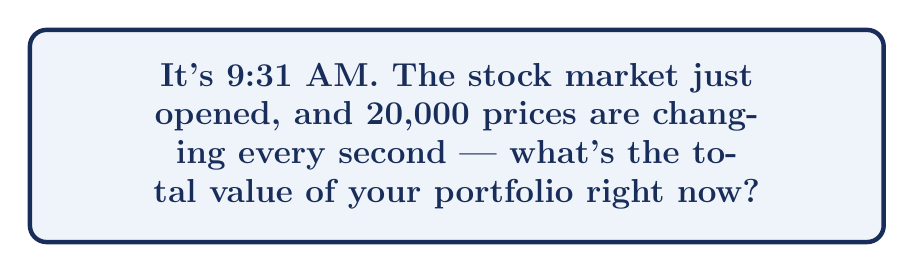
\begin{tikzpicture}[every node/.style={font=\small}]
  \node[draw=navy, ultra thick, fill=lightblue!30, rounded corners=6pt,
        text width=10cm, align=center, inner sep=12pt,
        font=\large\bfseries, text=navy]
        (q) {It's 9:31 AM. The stock market just opened, and 20{,}000 prices are changing every second --- what's the total value of your portfolio right now?};
\end{tikzpicture}
\vspace{0.4cm}
\pause
\begin{columns}[T]
\begin{column}{0.5\textwidth}
\centering
\textbf{\textcolor{warningred}{Recompute everything?}} \\[2pt]
\scriptsize Too slow when this happens thousands of times a second.
\end{column}
\pause
\begin{column}{0.5\textwidth}
\centering
\textbf{\textcolor{accentgreen}{Precompute once?}} \\[2pt]
\scriptsize Breaks the moment anything changes.
\end{column}
\end{columns}
\vspace{0.3cm}
\pause
\begin{block}{}
\centering This is the exact tension every large system --- stock feeds, leaderboards, analytics dashboards --- fights constantly.
\end{block}
\end{frame}

% ---------------- SLIDE 3: MAPPING + WHY THE OBVIOUS FIXES FAIL ----------------
\begin{frame}{From Wall Street to Array Indices}
\vspace{-0.1cm}
\begin{columns}[T]
\begin{column}{0.38\textwidth}
\small
\begin{block}{Translating the problem}
\begin{tabular}{@{}ll@{}}
Stock $i$'s price & $A[i]$ \\
Portfolio total & \texttt{sum(l,r)} \\
Price change & \texttt{update(i,v)} \\
\end{tabular}
\end{block}
\vspace{0.3cm}
\onslide<3->{
\begin{block}{The catch}
\small Keep the sum fresh $\Rightarrow$ every update is $O(n)$.\\
Keep updates instant $\Rightarrow$ every query is $O(n)$.
\end{block}}
\end{column}

\begin{column}{0.62\textwidth}
\centering
% ---- Stage 1: precomputed sum, watching stock i ----
\only<1>{
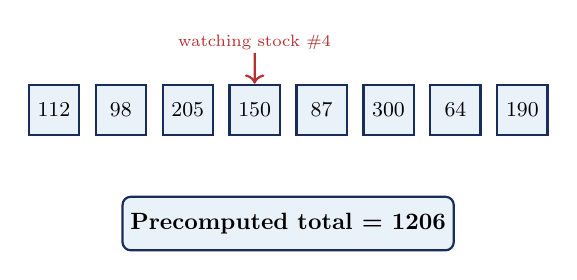
\begin{tikzpicture}[scale=0.85, every node/.style={transform shape}]
  \foreach \v [count=\i from 1] in {112,98,205,150,87,300,64,190}{
    \node[arrbox] (a\i) at (\i*1.0, 0) {\v};
  }
  \node[draw=navy, thick, fill=lightblue!40, rounded corners=3pt,
        minimum width=3.2cm, minimum height=0.8cm] (sum) at (4.5, -1.7) {\textbf{Precomputed total = 1206}};
  \node[font=\scriptsize, text=warningred] at (4, 1.0) {watching stock \#4};
  \draw[->, warningred, thick] (4, 0.85) -- (a4.north);
\end{tikzpicture}}
% ---- Stage 2: update hits, sum goes stale ----
\only<2>{
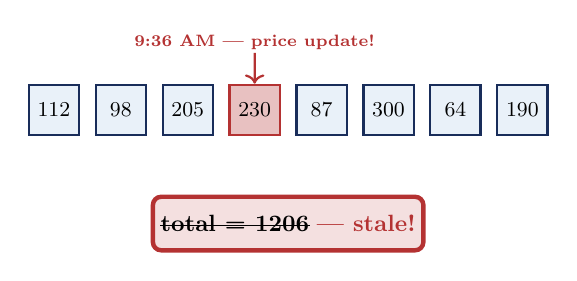
\begin{tikzpicture}[scale=0.85, every node/.style={transform shape}]
  \foreach \v [count=\i from 1] in {112,98,205,150,87,300,64,190}{
    \ifnum\i=4
      \node[arrbox, fill=warningred!30, draw=warningred] (a\i) at (\i*1.0, 0) {230};
    \else
      \node[arrbox] (a\i) at (\i*1.0, 0) {\v};
    \fi
  }
  \node[font=\scriptsize\bfseries, text=warningred] at (4, 1.0) {9:36 AM --- price update!};
  \draw[->, warningred, thick] (4, 0.85) -- (a4.north);
  \node[draw=warningred, ultra thick, fill=warningred!15, rounded corners=3pt,
        minimum width=3.4cm, minimum height=0.8cm] (sum) at (4.5, -1.7)
        {\sout{\textbf{total = 1206}} \textbf{\textcolor{warningred}{--- stale!}}};
\end{tikzpicture}}
% ---- Stage 3: both fixes cost O(n) ----
\only<3->{
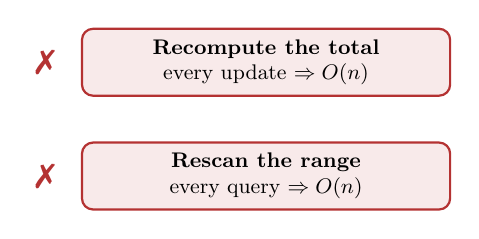
\begin{tikzpicture}[scale=0.85, every node/.style={transform shape}]
  \node[draw=warningred, thick, fill=warningred!10, rounded corners=4pt,
        minimum width=5.5cm, minimum height=1cm, align=center, font=\small]
        (o1) at (0,1.2) {\textbf{Recompute the total}\\ every update $\Rightarrow O(n)$};
  \node[draw=warningred, thick, fill=warningred!10, rounded corners=4pt,
        minimum width=5.5cm, minimum height=1cm, align=center, font=\small]
        (o2) at (0,-0.5) {\textbf{Rescan the range} \\ every query $\Rightarrow O(n)$};
  \node[font=\Large, text=warningred] at (-3.3, 1.2) {\ding{55}};
  \node[font=\Large, text=warningred] at (-3.3, -0.5) {\ding{55}};
\end{tikzpicture}}
\end{column}
\end{columns}
\end{frame}

% ---------------- SLIDE 4: THE DIVIDE-AND-CONQUER IDEA ----------------
\begin{frame}{What If We Just... Split the Problem?}
\centering
\vspace{0.4cm}
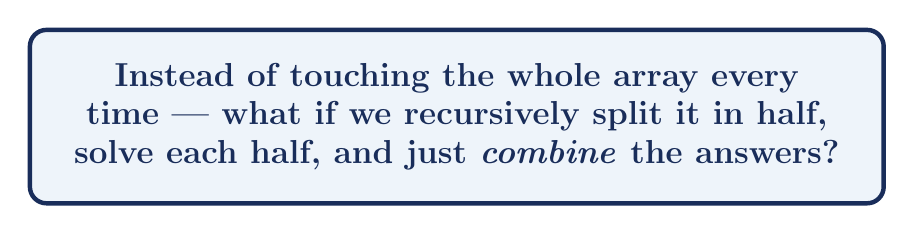
\begin{tikzpicture}[every node/.style={font=\small}]
  \node[draw=navy, ultra thick, fill=lightblue!30, rounded corners=6pt,
        text width=10cm, align=center, inner sep=12pt,
        font=\large\bfseries, text=navy]
        (q) {Instead of touching the whole array every time --- what if we recursively split it in half, solve each half, and just \emph{combine} the answers?};
\end{tikzpicture}
\vspace{0.5cm}
\pause
\begin{columns}[c]
\begin{column}{0.55\textwidth}
\begin{itemize}[<+->]\setlength{\itemsep}{4pt}
  \item Each split costs almost nothing.
  \item Only $O(\log n)$ splits are ever needed to reach any piece.
  \item Combining is cheap --- just merge two summaries.
\end{itemize}
\end{column}
\begin{column}{0.45\textwidth}
\centering
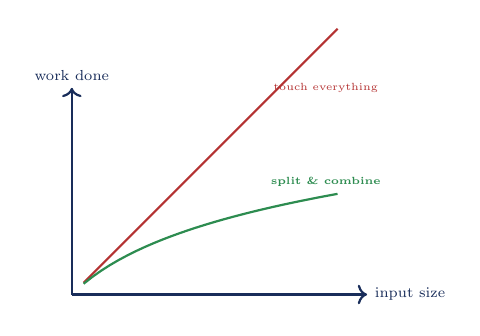
\begin{tikzpicture}[scale=0.75, every node/.style={transform shape, font=\scriptsize}]
  \onslide<5->{
  \draw[->, thick, navy] (0,0) -- (5,0) node[right] {input size};
  \draw[->, thick, navy] (0,0) -- (0,3.5) node[above] {work done};}
  \onslide<5->{\draw[thick, warningred] plot[domain=0.2:4.5, samples=30] (\x, {\x});}
  \onslide<5->{\node[text=warningred, font=\tiny] at (4.3,3.5) {touch everything};}
  \onslide<5->{\draw[thick, accentgreen] plot[domain=0.2:4.5, samples=30] (\x, {ln(\x+1)});}
  \onslide<5->{\node[text=accentgreen, font=\tiny\bfseries] at (4.3,1.9) {split \& combine};}
\end{tikzpicture}
\end{column}
\end{columns}
\vspace{0.3cm}
\onslide<6->{\centering\small That gap between the two curves --- \textbf{that's} the whole idea we're chasing.}
\end{frame}

% ---------------- SLIDE 5: COMPLEXITY GRAPH ----------------
\begin{frame}{Why $\log n$ Feels Free} 
\vspace{-0.1cm} \begin{center} 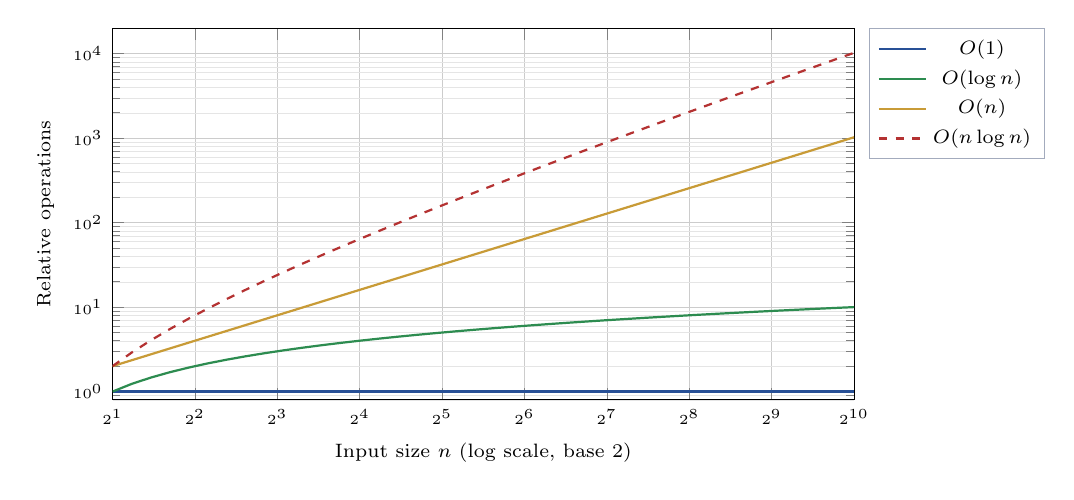
\begin{tikzpicture} \begin{axis}[ width=11cm, height=6.3cm, xlabel={Input size $n$ (log scale, base 2)}, ylabel={Relative operations}, xmode=log, log basis x=2, ymode=log, log basis y=10, xmin=2, xmax=1024, ymin=0.8, ymax=20000, grid=both, major grid style={line width=.2pt, draw=gray!40}, minor grid style={line width=.1pt, draw=gray!20}, legend style={at={(1.02,1)}, anchor=north west, font=\scriptsize, draw=navy!40}, every axis label/.append style={font=\scriptsize}, tick label style={font=\tiny}, ] \addplot[thick, deepblue, domain=2:1024, samples=40, mark=none] {1}; \addlegendentry{$O(1)$} \addplot[thick, accentgreen, domain=2:1024, samples=40, mark=none] {ln(x)/ln(2)}; \addlegendentry{$O(\log n)$} \addplot[thick, gold, domain=2:1024, samples=40, mark=none] {x}; \addlegendentry{$O(n)$} \addplot[thick, warningred, domain=2:1024, samples=40, mark=none, dashed] {x*ln(x)/ln(2)}; \addlegendentry{$O(n \log n)$} \end{axis} \end{tikzpicture} \end{center} \begin{center}\scriptsize \textcolor{accentgreen}{$\log_2 n$ grows glacially --- e.g.\ $\log_2 (10^9) \approx 30$.} \end{center} 
\end{frame}



% ---------------- SLIDE 6: CORE IDEA ----------------
\begin{frame}{Split It, Store It, Solve It}
\small
Store a \bignav{summary} of each interval at a tree node; queries \textbf{glue} summaries together.
\vspace{-0.1cm}
\begin{center}
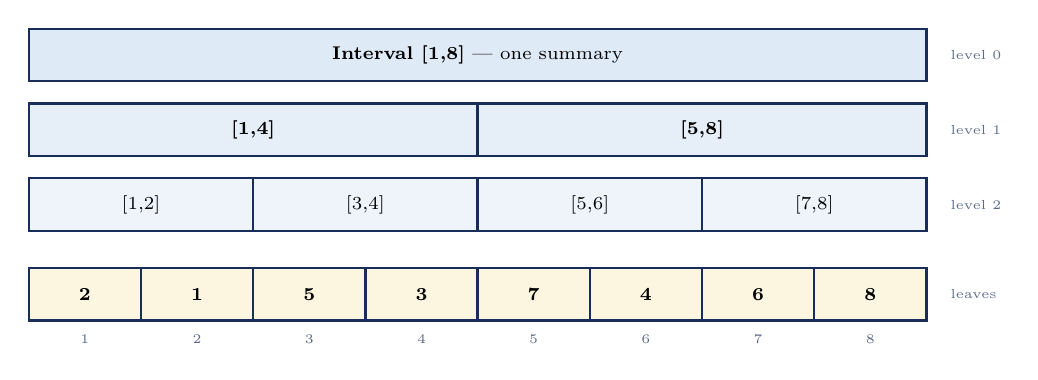
\begin{tikzpicture}[scale=0.95, every node/.style={transform shape, font=\scriptsize}]
  \draw[navy, thick, fill=lightblue!60] (0,3.6) rectangle (12,4.3);
  \node at (6, 3.95) {\textbf{Interval [1,8]} --- one summary};

  \onslide<2->{
  \draw[navy, thick, fill=lightblue!45] (0,2.6) rectangle (6,3.3);
  \node at (3, 2.95) {\textbf{[1,4]}};
  \draw[navy, thick, fill=lightblue!45] (6,2.6) rectangle (12,3.3);
  \node at (9, 2.95) {\textbf{[5,8]}};
  }

  \onslide<3->{
  \foreach \i/\l/\r in {0/1/2, 3/3/4, 6/5/6, 9/7/8}{
    \draw[navy, thick, fill=lightblue!30] (\i,1.6) rectangle (\i+3,2.3);
    \node at (\i+1.5, 1.95) {[\l,\r]};
  }
  }

  \onslide<4->{
  \foreach \i/\v/\idx in {0/2/1, 1.5/1/2, 3/5/3, 4.5/3/4, 6/7/5, 7.5/4/6, 9/6/7, 10.5/8/8}{
    \draw[navy, thick, fill=cream] (\i,0.4) rectangle (\i+1.5,1.1);
    \node at (\i+0.75, 0.75) {\textbf{\v}};
    \node[font=\tiny, text=navy!70] at (\i+0.75, 0.15) {\idx};
  }
  }

  \node[font=\tiny, text=navy!70, anchor=west] at (12.2, 3.95) {level 0};
  \onslide<2->{\node[font=\tiny, text=navy!70, anchor=west] at (12.2, 2.95) {level 1};}
  \onslide<3->{\node[font=\tiny, text=navy!70, anchor=west] at (12.2, 1.95) {level 2};}
  \onslide<4->{\node[font=\tiny, text=navy!70, anchor=west] at (12.2, 0.75) {leaves};}
\end{tikzpicture}
\end{center}
\onslide<5->
\begin{itemize}[<+->]\setlength{\itemsep}{1pt}
  \item Children split each interval in half; height $=\lceil \log_2 n \rceil$.
  \item Any range $[l,r]$ decomposes into just $O(\log n)$ pieces.
\end{itemize}
\end{frame}

% ---------------- SLIDE: ANATOMY ---------------- 
\begin{frame}{Build Segment Tree} \vspace{-0.15cm} 
\begin{center} 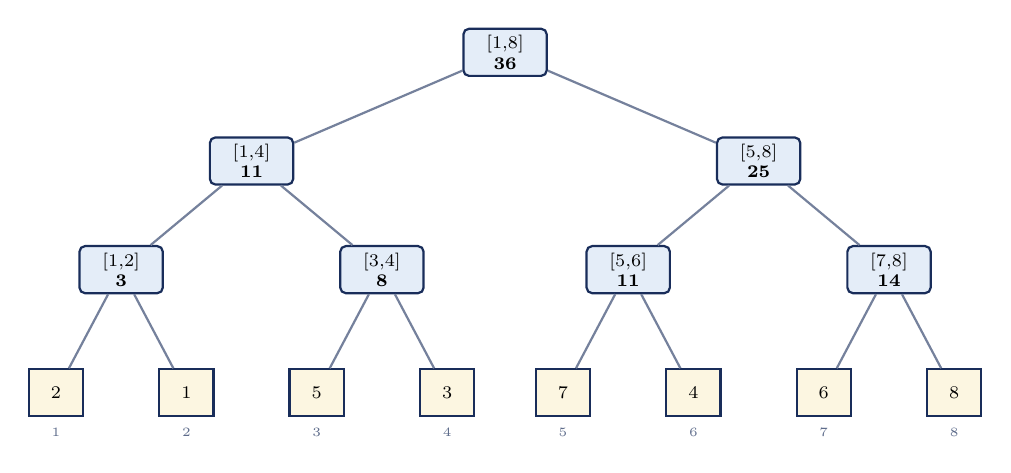
\begin{tikzpicture}[scale=0.92, every node/.style={transform shape}] \onslide<4->{\node[segnode] (n1) at (7, 6) {[1,8]\\ \textbf{36}};} \onslide<3->{ \node[segnode] (n2) at (3.5, 4.5) {[1,4]\\ \textbf{11}}; \node[segnode] (n3) at (10.5, 4.5) {[5,8]\\ \textbf{25}};} \onslide<2->{ \node[segnode] (n4) at (1.7, 3) {[1,2]\\ \textbf{3}}; \node[segnode] (n5) at (5.3, 3) {[3,4]\\ \textbf{8}}; \node[segnode] (n6) at (8.7, 3) {[5,6]\\ \textbf{11}}; \node[segnode] (n7) at (12.3, 3) {[7,8]\\ \textbf{14}};} \node[segleaf] (l1) at (0.8, 1.3) {2}; \node[segleaf] (l2) at (2.6, 1.3) {1}; \node[segleaf] (l3) at (4.4, 1.3) {5}; \node[segleaf] (l4) at (6.2, 1.3) {3}; \node[segleaf] (l5) at (7.8, 1.3) {7}; \node[segleaf] (l6) at (9.6, 1.3) {4}; \node[segleaf] (l7) at (11.4, 1.3) {6}; \node[segleaf] (l8) at (13.2, 1.3) {8}; \onslide<2->{\draw[segedge] (n4)--(l1); \draw[segedge] (n4)--(l2); \draw[segedge] (n5)--(l3); \draw[segedge] (n5)--(l4); \draw[segedge] (n6)--(l5); \draw[segedge] (n6)--(l6); \draw[segedge] (n7)--(l7); \draw[segedge] (n7)--(l8);} \onslide<3->{\draw[segedge] (n2)--(n4); \draw[segedge] (n2)--(n5); \draw[segedge] (n3)--(n6); \draw[segedge] (n3)--(n7);} \onslide<4->{\draw[segedge] (n1)--(n2); \draw[segedge] (n1)--(n3);} \foreach \x/\i in {0.8/1, 2.6/2, 4.4/3, 6.2/4, 7.8/5, 9.6/6, 11.4/7, 13.2/8} \node[font=\tiny, text=navy!70] at (\x, 0.75) {\i}; \end{tikzpicture} \end{center} \onslide<5->{\centering\small Built bottom-up: each parent is just the \bignav{merge} of its two children.} 
\end{frame}


% PART II -- RANGE QUERY & POINT UPDATE (Shayan)
% ============================================================
\setpresenter{Shayan --- Problem \& Application}
\section{Part II --- Range Query \& Point Update}

% ---------------- SLIDE: UPDATE LOGIC ----------------
\begin{frame}{Finding the Target: Which Way Do We Go?}
\centering
\vspace{0.15cm}
\small
To update index $i$, a node only needs to know \textbf{one thing}: does $i$ fall in its left half or its right half?
\vspace{0.3cm}

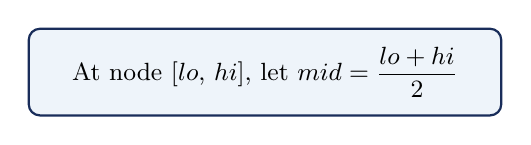
\begin{tikzpicture}[every node/.style={font=\small}, node distance=1.4cm]
  \onslide<1->{
  \node[draw=navy, thick, fill=lightblue!30, rounded corners=4pt,
        minimum width=6cm, minimum height=1.1cm, align=center] (mid)
        {At node [$lo$, $hi$], let $mid = \dfrac{lo+hi}{2}$};}
\end{tikzpicture}
\vspace{0.35cm}

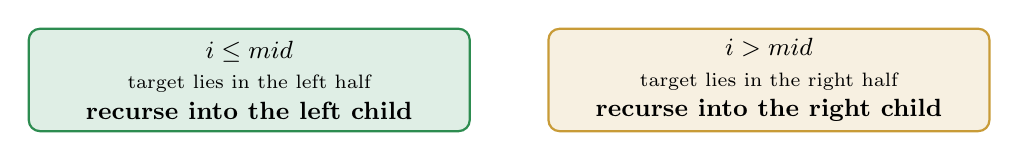
\begin{tikzpicture}[every node/.style={font=\small}, node distance=1.2cm]
  \onslide<2->{
  \node[draw=accentgreen, thick, fill=softgreen, rounded corners=4pt,
        minimum width=5.6cm, minimum height=1.3cm, align=center] (c1) at (-3.3,0)
    {\textbf{$i \le mid$}\\ \scriptsize target lies in the left half\\ \textbf{recurse into the left child}};}
  \onslide<3->{
  \node[draw=gold, thick, fill=gold!15, rounded corners=4pt,
        minimum width=5.6cm, minimum height=1.3cm, align=center] (c2) at (3.3,0)
    {\textbf{$i > mid$}\\ \scriptsize target lies in the right half\\ \textbf{recurse into the right child}};}
\end{tikzpicture}
\vspace{0.35cm}

\onslide<4->{\small Exactly \textbf{one} child is ever visited at each level --- never both --- until a single leaf, index $i$ itself, is reached.}
\end{frame}

% ---------------- SLIDE: UPDATE WALKTHROUGH ----------------
\begin{frame}{One Change, $\log n$ Fixes: update(4, 10)}
\begin{tikzpicture}[remember picture, overlay]
\node[anchor=north west] at ([xshift=0.4cm, yshift=-1.6cm]current page.north west) {%
\only<1-3>{%
\begin{tikzpicture}[scale=0.65, every node/.style={transform shape}]
  \foreach \v/\i in {2/1,1/2,5/3,3/4,7/5,4/6,6/7,8/8}{
    \pgfmathsetmacro{\x}{(\i-1)*0.85}
    \ifnum\i=4
      \draw[warningred, thick, fill=warningred!15] (\x,0) rectangle (\x+0.75,0.75);
    \else
      \draw[navy, thick, fill=lightblue!30] (\x,0) rectangle (\x+0.75,0.75);
    \fi
    \node[anchor=center, font=\large] at (\x+0.375,0.375) {\v};
    \node[anchor=center, font=\normalsize, text=navy!60] at (\x+0.375,-0.28) {\i};
  }
\end{tikzpicture}%
}%
\only<4->{%
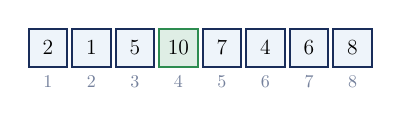
\begin{tikzpicture}[scale=0.65, every node/.style={transform shape}]
  \foreach \v/\i in {2/1,1/2,5/3,10/4,7/5,4/6,6/7,8/8}{
    \pgfmathsetmacro{\x}{(\i-1)*0.85}
    \ifnum\i=4
      \draw[accentgreen, thick, fill=softgreen] (\x,0) rectangle (\x+0.75,0.75);
    \else
      \draw[navy, thick, fill=lightblue!30] (\x,0) rectangle (\x+0.75,0.75);
    \fi
    \node[anchor=center, font=\large] at (\x+0.375,0.375) {\v};
    \node[anchor=center, font=\normalsize, text=navy!60] at (\x+0.375,-0.28) {\i};
  }
\end{tikzpicture}%
}%
};
\end{tikzpicture}
\vspace{-0.25cm}
\begin{center}
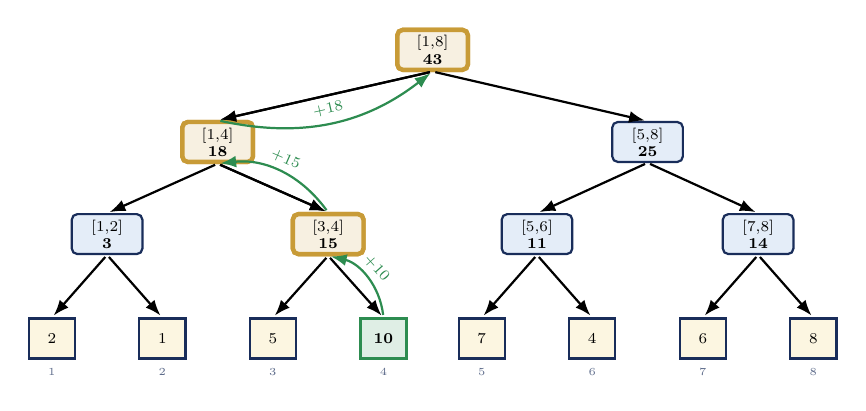
\begin{tikzpicture}[scale=0.78, every node/.style={transform shape}]

  % ---- STEP 1: root, in-range, not yet resolved ----
  \onslide<1-6>{\node[segnode, segpath] (n1) at (7,6) {[1,8]\\ \textbf{36}};}
  \onslide<7->{\node[segnode, segpath] (n1b) at (7,6) {[1,8]\\ \textbf{43}};}

  % ---- STEP 2: [1,4], in-range, descend ----
  \onslide<2-5>{
    \node[segnode, segpath] (n2) at (3.5,4.5) {[1,4]\\ \textbf{11}};
    \draw[-{Latex[length=2mm]}, thick, black, shorten >=1pt, shorten <=1pt] (n1.south) -- (n2.north);
  }
  \onslide<6->{
    \node[segnode, segpath] (n2b) at (3.5,4.5) {[1,4]\\ \textbf{18}};
    \draw[-{Latex[length=2mm]}, thick, black, shorten >=1pt, shorten <=1pt] (n1.south) -- (n2b.north);
  }

  % ---- STEP 3: [3,4], in-range, descend ----
  \onslide<3-4>{
    \node[segnode, segpath] (n5) at (5.3,3) {[3,4]\\ \textbf{8}};
    \draw[-{Latex[length=2mm]}, thick, black, shorten >=1pt, shorten <=1pt] (n2.south) -- (n5.north);
  }
  \onslide<5->{
    \node[segnode, segpath] (n5b) at (5.3,3) {[3,4]\\ \textbf{15}};
    \draw[-{Latex[length=2mm]}, thick, black, shorten >=1pt, shorten <=1pt] (n2.south) -- (n5b.north);
  }

  % ---- STEP 4: leaf 4, target index reached ----
  \onslide<4->{
    \node[segleaf, segfull] (l4) at (6.2,1.3) {\textbf{10}};
    \draw[-{Latex[length=2mm]}, thick, black, shorten >=1pt, shorten <=1pt] (n5.south) -- (l4.north);
  }

  % ---- STEP 5: sibling leaf 3, revealed with black edge + curved green return ----
  \onslide<5->{
    \node[segleaf] (l3) at (4.4,1.3) {5};
    \draw[-{Latex[length=2mm]}, thick, black, shorten >=1pt, shorten <=1pt] (n5b.south) -- (l3.north);
    \draw[-{Latex[length=2mm]}, thick, accentgreen, bend right=35, shorten >=1pt, shorten <=1pt]
      (l4.north) to node[midway, sloped, above, font=\scriptsize\bfseries, text=accentgreen]{$+10$} (n5b.south);
  }

  % ---- STEP 6: sibling subtree [1,2], revealed with black edges + curved green return ----
  \onslide<6->{
    \node[segnode] (n4) at (1.7,3) {[1,2]\\ \textbf{3}};
    \node[segleaf] (l1) at (0.8,1.3) {2};
    \node[segleaf] (l2) at (2.6,1.3) {1};
    \draw[-{Latex[length=2mm]}, thick, black, shorten >=1pt, shorten <=1pt] (n2b.south) -- (n4.north);
    \draw[-{Latex[length=2mm]}, thick, black, shorten >=1pt, shorten <=1pt] (n4.south) -- (l1.north);
    \draw[-{Latex[length=2mm]}, thick, black, shorten >=1pt, shorten <=1pt] (n4.south) -- (l2.north);
    \draw[-{Latex[length=2mm]}, thick, accentgreen, bend right=30, shorten >=1pt, shorten <=1pt]
      (n5b.north) to node[midway, sloped, above, font=\scriptsize\bfseries, text=accentgreen]{$+15$} (n2b.south);
  }

  % ---- STEP 7: entire right subtree [5,8], revealed + curved green return to root ----
  \onslide<7->{
    \node[segnode] (n3) at (10.5,4.5) {[5,8]\\ \textbf{25}};
    \node[segnode] (n6) at (8.7,3) {[5,6]\\ \textbf{11}};
    \node[segnode] (n7) at (12.3,3) {[7,8]\\ \textbf{14}};
    \node[segleaf] (l5) at (7.8,1.3) {7};
    \node[segleaf] (l6) at (9.6,1.3) {4};
    \node[segleaf] (l7) at (11.4,1.3) {6};
    \node[segleaf] (l8) at (13.2,1.3) {8};
    \draw[-{Latex[length=2mm]}, thick, black, shorten >=1pt, shorten <=1pt] (n1b.south) -- (n3.north);
    \draw[-{Latex[length=2mm]}, thick, black, shorten >=1pt, shorten <=1pt] (n3.south) -- (n6.north);
    \draw[-{Latex[length=2mm]}, thick, black, shorten >=1pt, shorten <=1pt] (n3.south) -- (n7.north);
    \draw[-{Latex[length=2mm]}, thick, black, shorten >=1pt, shorten <=1pt] (n6.south) -- (l5.north);
    \draw[-{Latex[length=2mm]}, thick, black, shorten >=1pt, shorten <=1pt] (n6.south) -- (l6.north);
    \draw[-{Latex[length=2mm]}, thick, black, shorten >=1pt, shorten <=1pt] (n7.south) -- (l7.north);
    \draw[-{Latex[length=2mm]}, thick, black, shorten >=1pt, shorten <=1pt] (n7.south) -- (l8.north);
    \draw[-{Latex[length=2mm]}, thick, accentgreen, bend right=25, shorten >=1pt, shorten <=1pt]
      (n2b.north) to node[midway, sloped, above, font=\scriptsize\bfseries, text=accentgreen]{$+18$} (n1b.south);
  }

  \foreach \x/\i in {0.8/1, 2.6/2, 4.4/3, 6.2/4, 7.8/5, 9.6/6, 11.4/7, 13.2/8}
    \node[font=\tiny, text=navy!70] at (\x, 0.75) {\i};
\end{tikzpicture}
\end{center}
\onslide<8->{\centering\small \textbf{Black} = descending to the target index. \textbf{Green} = merging back up. Only $\log n$ nodes ever touched.}
\onslide<8->{
\vspace{3pt}
\begin{center}

\begin{tikzpicture}
\node[draw=accentgreen, thick, fill=softgreen, rounded corners=3pt, inner sep=5pt, font=\scriptsize\bfseries, text=accentgreen!60!black]
  {update(i, v) costs exactly $O(\log n)$ --- one downward pass, one upward merge};
\end{tikzpicture}
\end{center}
}
\end{frame}

% ---------------- SLIDE: UPDATE TIME COMPLEXITY ----------------
\begin{frame}{Time Complexity of update()}
\vspace{-0.1cm}
\centering
\small
An update walks exactly \textbf{one path}: root $\to$ target leaf, then merges its way back up along that very same path.
\vspace{0.2cm}

\par
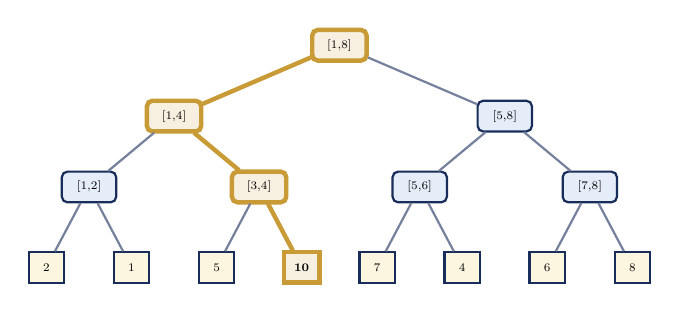
\begin{tikzpicture}[scale=0.60, every node/.style={transform shape}]
  \node[segnode, segpath] (n1) at (7,6) {[1,8]};
  \node[segnode] (n2o) at (10.5,4.5) {[5,8]};
  \node[segnode, segpath] (n2) at (3.5,4.5) {[1,4]};
  \node[segnode] (n4o) at (1.7,3) {[1,2]};
  \node[segnode, segpath] (n5) at (5.3,3) {[3,4]};
  \node[segnode] (n6o) at (8.7,3) {[5,6]};
  \node[segnode] (n7o) at (12.3,3) {[7,8]};
  \node[segleaf] (l1) at (0.8,1.3) {2};
  \node[segleaf] (l2) at (2.6,1.3) {1};
  \node[segleaf] (l3) at (4.4,1.3) {5};
  \node[segleaf, segpath] (l4) at (6.2,1.3) {\textbf{10}};
  \node[segleaf] (l5) at (7.8,1.3) {7};
  \node[segleaf] (l6) at (9.6,1.3) {4};
  \node[segleaf] (l7) at (11.4,1.3) {6};
  \node[segleaf] (l8) at (13.2,1.3) {8};
  \draw[segedge] (n1)--(n2o);
  \draw[segedge] (n2o)--(n6o); \draw[segedge] (n2o)--(n7o);
  \draw[segedge] (n2)--(n4o);
  \draw[segedge] (n4o)--(l1); \draw[segedge] (n4o)--(l2);
  \draw[segedge] (n5)--(l3);
  \draw[segedge] (n6o)--(l5); \draw[segedge] (n6o)--(l6);
  \draw[segedge] (n7o)--(l7); \draw[segedge] (n7o)--(l8);
  \draw[segedgeactive] (n1)--(n2);
  \draw[segedgeactive] (n2)--(n5);
  \draw[segedgeactive] (n5)--(l4);
\end{tikzpicture}
\par

\begin{itemize}\setlength{\itemsep}{3pt}
  \item Going down: one node chosen per level --- left \emph{or} right child, never both.
  \item Coming back up: one merge per level, along that same path.
  \item Total work $\propto$ number of levels visited $=$ \textbf{height of the tree}.
\end{itemize}
\vspace{0.1cm}
A segment tree built on $n$ leaves is a \textbf{full binary tree}, so its height is $\lceil \log_2 n\rceil$.
\vspace{0.15cm}
\par

\begin{tikzpicture}
\node[draw=accentgreen, ultra thick, fill=softgreen, rounded corners=5pt, inner sep=7pt, font=\large\bfseries, text=accentgreen!60!black]
  {update(i, v) $= O(\log n)$};
\end{tikzpicture}
\par
\end{frame}

% ---------------- SLIDE: THREE CASES ----------------
\begin{frame}{Answering sum(l, r): Three Cases, Nothing Else}
\centering
\vspace{0.15cm}
\small
Every node compares its own range $[lo, hi]$ against the query range $[l, r]$ --- exactly one of three cases applies:
\vspace{0.25cm}

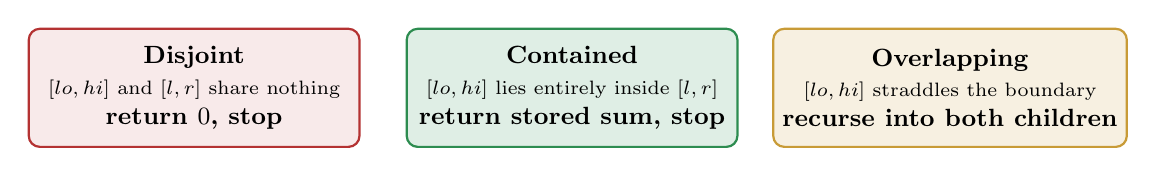
\begin{tikzpicture}[every node/.style={font=\small}, node distance=1.2cm]
  \onslide<1->{
  \node[draw=warningred, thick, fill=warningred!10, rounded corners=4pt,
        minimum width=4.2cm, minimum height=1.5cm, align=center] (c1) at (-4.8,0)
    {\textbf{Disjoint}\\ \scriptsize $[lo,hi]$ and $[l,r]$ share nothing\\ \textbf{return $0$, stop}};}
  \onslide<2->{
  \node[draw=accentgreen, thick, fill=softgreen, rounded corners=4pt,
        minimum width=4.2cm, minimum height=1.5cm, align=center] (c2) at (0,0)
    {\textbf{Contained}\\ \scriptsize $[lo,hi]$ lies entirely inside $[l,r]$\\ \textbf{return stored sum, stop}};}
  \onslide<3->{
  \node[draw=gold, thick, fill=gold!15, rounded corners=4pt,
        minimum width=4.2cm, minimum height=1.5cm, align=center] (c3) at (4.8,0)
    {\textbf{Overlapping}\\ \scriptsize $[lo,hi]$ straddles the boundary\\ \textbf{recurse into both children}};}
\end{tikzpicture}
\vspace{0.4cm}

\onslide<3->{\small Only the \textbf{Overlapping} case ever recurses further --- and at most $2$ such nodes exist per level.}
\end{frame}

% ---------------- SLIDE: QUERY WALKTHROUGH (SIGNATURE) ----------------
\begin{frame}{Watching sum(3,7) Unfold --- On the Updated Array}
\begin{tikzpicture}[remember picture, overlay]
\node[anchor=north west] at ([xshift=0.4cm, yshift=-1.6cm]current page.north west) {%
\begin{tikzpicture}[scale=0.65, every node/.style={transform shape}]
  \foreach \v/\i in {2/1,1/2,5/3,10/4,7/5,4/6,6/7,8/8}{
    \pgfmathsetmacro{\x}{(\i-1)*0.85}
    \ifnum\i>2
      \ifnum\i<8
        \onslide<12->{\draw[accentgreen, thick, fill=softgreen] (\x,0) rectangle (\x+0.75,0.75);}
        \onslide<1-11>{\draw[gold, ultra thick, fill=lightblue!30] (\x,0) rectangle (\x+0.75,0.75);}
      \else
        \draw[navy, thick, fill=lightblue!30] (\x,0) rectangle (\x+0.75,0.75);
      \fi
    \else
      \draw[navy, thick, fill=lightblue!30] (\x,0) rectangle (\x+0.75,0.75);
    \fi
    \node[anchor=center, font=\large] at (\x+0.375,0.375) {\v};
    \node[anchor=center, font=\normalsize, text=navy!60] at (\x+0.375,-0.28) {\i};
  }
  \onslide<12->{
    \draw[overlay, accentgreen, thick, decorate, decoration={brace, amplitude=3pt}]
      (1.7,0.9) -- (5.85,0.9)
      node[midway, above=5pt, font=\large\bfseries, text=accentgreen!60!black] {$\mathrm{sum} = 32$};
  }
\end{tikzpicture}%
};
\end{tikzpicture}
\vspace{-0.2cm}
\begin{center}
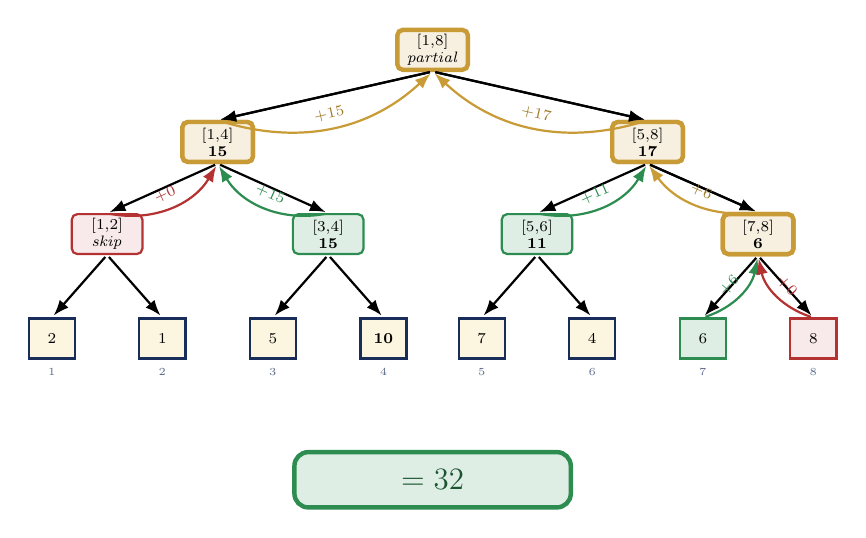
\begin{tikzpicture}[scale=0.78, every node/.style={transform shape}]

  % ---- STEP 1: root, partial ----
  \onslide<1->{\node[segnode, segpath] (n1) at (7,6) {[1,8]\\ \textit{partial}};}

  % ---- STEP 2: [1,4], partial, descend (black) ----
  \onslide<2-4>{
    \node[segnode, segpath] (n2) at (3.5,4.5) {[1,4]\\ \textit{partial}};
    \draw[-{Latex[length=2mm]}, thick, black, shorten >=1pt, shorten <=1pt] (n1.south) -- (n2.north);
  }
  \onslide<5->{
    \node[segnode, segpath] (n2r) at (3.5,4.5) {[1,4]\\ \textbf{15}};
    \draw[-{Latex[length=2mm]}, thick, black, shorten >=1pt, shorten <=1pt] (n1.south) -- (n2r.north);
  }

  % ---- STEP 3: [1,2], no overlap, descend (black) then red return ----
  \onslide<3->{
    \node[segnode, segskip] (n4) at (1.7,3) {[1,2]\\ \textit{skip}};
    \node[segleaf] (l1) at (0.8,1.3) {2};
    \node[segleaf] (l2) at (2.6,1.3) {1};
    \draw[-{Latex[length=2mm]}, thick, black, shorten >=1pt, shorten <=1pt] (n4.south) -- (l1.north);
    \draw[-{Latex[length=2mm]}, thick, black, shorten >=1pt, shorten <=1pt] (n4.south) -- (l2.north);
    \draw[-{Latex[length=2mm]}, thick, black, shorten >=1pt, shorten <=1pt] (n2.south) -- (n4.north);
    \draw[-{Latex[length=2mm]}, thick, warningred, bend right=35, shorten >=1pt, shorten <=1pt]
      (n4.north) to node[midway, sloped, above, font=\scriptsize\bfseries, text=warningred]{$+0$} (n2.south);
  }

  % ---- STEP 4: [3,4], full overlap, descend (black) then green return ----
  \onslide<4->{
    \node[segnode, segfull] (n5) at (5.3,3) {[3,4]\\ \textbf{15}};
    \node[segleaf] (l3) at (4.4,1.3) {5};
    \node[segleaf] (l4) at (6.2,1.3) {\textbf{10}};
    \draw[-{Latex[length=2mm]}, thick, black, shorten >=1pt, shorten <=1pt] (n5.south) -- (l3.north);
    \draw[-{Latex[length=2mm]}, thick, black, shorten >=1pt, shorten <=1pt] (n5.south) -- (l4.north);
    \draw[-{Latex[length=2mm]}, thick, black, shorten >=1pt, shorten <=1pt] (n2.south) -- (n5.north);
    \draw[-{Latex[length=2mm]}, thick, accentgreen, bend left=35, shorten >=1pt, shorten <=1pt]
      (n5.north) to node[midway, sloped, above, font=\scriptsize\bfseries, text=accentgreen]{$+15$} (n2.south);
  }

  % ---- STEP 5: [1,4] resolves, gold return to root ----
  \onslide<5->{
    \draw[-{Latex[length=2mm]}, thick, gold, bend right=30, shorten >=1pt, shorten <=1pt]
      (n2r.north) to node[midway, sloped, above, font=\scriptsize\bfseries, text=darkgold]{$+15$} (n1.south);
  }

  % ---- STEP 6: [5,8], partial, descend (black) ----
  \onslide<6-10>{
    \node[segnode, segpath] (n3) at (10.5,4.5) {[5,8]\\ \textit{partial}};
    \draw[-{Latex[length=2mm]}, thick, black, shorten >=1pt, shorten <=1pt] (n1.south) -- (n3.north);
  }
  \onslide<11->{
    \node[segnode, segpath] (n3r) at (10.5,4.5) {[5,8]\\ \textbf{17}};
    \draw[-{Latex[length=2mm]}, thick, black, shorten >=1pt, shorten <=1pt] (n1.south) -- (n3r.north);
  }

  % ---- STEP 7: [5,6], full overlap, descend (black) then green return ----
  \onslide<7->{
    \node[segnode, segfull] (n6) at (8.7,3) {[5,6]\\ \textbf{11}};
    \node[segleaf] (l5) at (7.8,1.3) {7};
    \node[segleaf] (l6) at (9.6,1.3) {4};
    \draw[-{Latex[length=2mm]}, thick, black, shorten >=1pt, shorten <=1pt] (n6.south) -- (l5.north);
    \draw[-{Latex[length=2mm]}, thick, black, shorten >=1pt, shorten <=1pt] (n6.south) -- (l6.north);
    \draw[-{Latex[length=2mm]}, thick, black, shorten >=1pt, shorten <=1pt] (n3.south) -- (n6.north);
    \draw[-{Latex[length=2mm]}, thick, accentgreen, bend right=35, shorten >=1pt, shorten <=1pt]
      (n6.north) to node[midway, sloped, above, font=\scriptsize\bfseries, text=accentgreen]{$+11$} (n3.south);
  }

  % ---- STEP 8: [7,8], partial, descend (black) ----
  \onslide<8-9>{
    \node[segnode, segpath] (n7) at (12.3,3) {[7,8]\\ \textit{partial}};
    \draw[-{Latex[length=2mm]}, thick, black, shorten >=1pt, shorten <=1pt] (n3.south) -- (n7.north);
  }
  \onslide<10->{
    \node[segnode, segpath] (n7r) at (12.3,3) {[7,8]\\ \textbf{6}};
    \draw[-{Latex[length=2mm]}, thick, black, shorten >=1pt, shorten <=1pt] (n3.south) -- (n7r.north);
  }

  % ---- STEP 9: leaf 7 (full, green) and leaf 8 (skip, red), both descend + return ----
  \onslide<9->{
    \node[segleaf, segfull] (l7) at (11.4,1.3) {6};
    \node[segleaf, segskip] (l8) at (13.2,1.3) {8};
    \draw[-{Latex[length=2mm]}, thick, black, shorten >=1pt, shorten <=1pt] (n7.south) -- (l7.north);
    \draw[-{Latex[length=2mm]}, thick, black, shorten >=1pt, shorten <=1pt] (n7.south) -- (l8.north);
    \draw[-{Latex[length=2mm]}, thick, accentgreen, bend right=30, shorten >=1pt, shorten <=1pt]
      (l7.north) to node[midway, sloped, above, font=\scriptsize\bfseries, text=accentgreen]{$+6$} (n7.south);
    \draw[-{Latex[length=2mm]}, thick, warningred, bend left=30, shorten >=1pt, shorten <=1pt]
      (l8.north) to node[midway, sloped, above, font=\scriptsize\bfseries, text=warningred]{$+0$} (n7.south);
  }

  % ---- STEP 10: [7,8] resolves, gold return to [5,8] ----
  \onslide<10->{
    \draw[-{Latex[length=2mm]}, thick, gold, bend left=30, shorten >=1pt, shorten <=1pt]
      (n7r.north) to node[midway, sloped, above, font=\scriptsize\bfseries, text=darkgold]{$+6$} (n3.south);
  }

  % ---- STEP 11: [5,8] resolves, gold return to root ----
  \onslide<11->{
    \draw[-{Latex[length=2mm]}, thick, gold, bend left=30, shorten >=1pt, shorten <=1pt]
      (n3r.north) to node[midway, sloped, above, font=\scriptsize\bfseries, text=darkgold]{$+17$} (n1.south);
  }

  \foreach \x/\i in {0.8/1, 2.6/2, 4.4/3, 6.2/4, 7.8/5, 9.6/6, 11.4/7, 13.2/8}
    \node[font=\tiny, text=navy!70] at (\x, 0.75) {\i};

  % ---- Running total, builds left to right as each meaningful return lands ----
  \onslide<3>{\node[font=\Large, text=navy] at (7,-1) {$0$};}
  \onslide<4-6>{\node[font=\Large, text=navy] at (7,-1) {$0 + 15$};}
  \onslide<7-8>{\node[font=\Large, text=navy] at (7,-1) {$0 + 15 + 11$};}
  \onslide<9-11>{\node[font=\Large, text=navy] at (7,-1) {$0 + 15 + 11 + 6 + 0$};}
  \onslide<12->{
    \node[draw=accentgreen, ultra thick, fill=softgreen, rounded corners=5pt,
          minimum width=4.5cm, minimum height=0.9cm, font=\Large\bfseries, text=accentgreen!60!black]
          at (7,-1) {$= 32$};
  }
\end{tikzpicture}
\end{center}
\onslide<12->{
\vspace{-2pt}
{\centering\scriptsize\textcolor{navy!70}{Cells 3--7 in the array above (highlighted green) sum to exactly \textbf{32} --- confirming the tree's answer. Only \textbf{7} of the tree's 15 nodes were ever visited.}\par}
}
\end{frame}

% ---------------- SLIDE: QUERY TIME COMPLEXITY ----------------
\begin{frame}{Time Complexity of sum(l, r): The Overlap Argument}
\small
At \textbf{every level}, the query boundary can cut through at most \textbf{one} segment on the left and \textbf{one} on the right --- everything else is fully in or fully out.
\vspace{-0.05cm}
\begin{center}
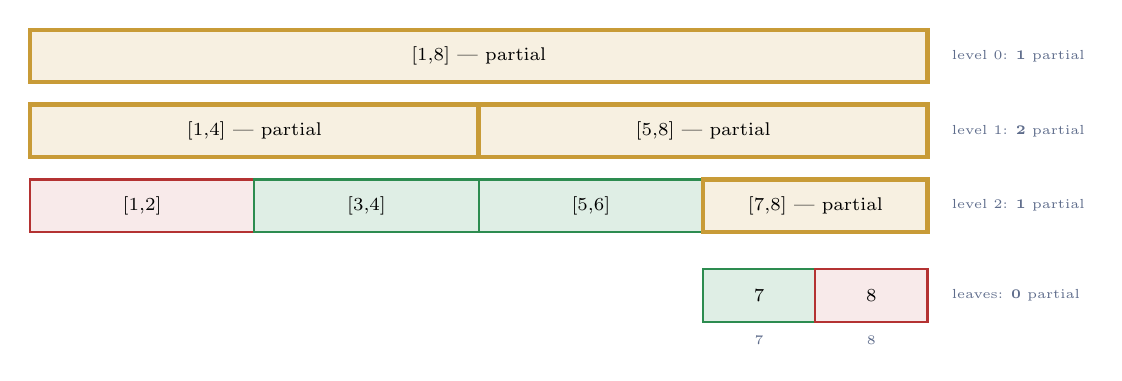
\begin{tikzpicture}[scale=0.95, every node/.style={transform shape, font=\scriptsize}]
  % Level 0 -- root
  \onslide<1->{
  \draw[gold, ultra thick, fill=gold!15] (0,3.6) rectangle (12,4.3);
  \node at (6,3.95) {[1,8] --- partial};
  }
  % Level 1
  \onslide<2->{
  \draw[gold, ultra thick, fill=gold!15] (0,2.6) rectangle (6,3.3);
  \node at (3,2.95) {[1,4] --- partial};
  \draw[gold, ultra thick, fill=gold!15] (6,2.6) rectangle (12,3.3);
  \node at (9,2.95) {[5,8] --- partial};
  }
  % Level 2
  \onslide<3->{
  \draw[warningred, thick, fill=warningred!10] (0,1.6) rectangle (3,2.3);
  \node at (1.5,1.95) {[1,2]};
  \draw[accentgreen, thick, fill=softgreen] (3,1.6) rectangle (6,2.3);
  \node at (4.5,1.95) {[3,4]};
  \draw[accentgreen, thick, fill=softgreen] (6,1.6) rectangle (9,2.3);
  \node at (7.5,1.95) {[5,6]};
  \draw[gold, ultra thick, fill=gold!15] (9,1.6) rectangle (12,2.3);
  \node at (10.5,1.95) {[7,8] --- partial};
  }
  % Leaves -- only the still-partial [7,8] needs to split further
  \onslide<4->{
  \draw[accentgreen, thick, fill=softgreen] (9,0.4) rectangle (10.5,1.1);
  \node at (9.75,0.75) {7};
  \draw[warningred, thick, fill=warningred!10] (10.5,0.4) rectangle (12,1.1);
  \node at (11.25,0.75) {8};
  \node[font=\tiny, text=navy!70] at (9.75,0.15) {7};
  \node[font=\tiny, text=navy!70] at (11.25,0.15) {8};
  }

  \node[font=\tiny, text=navy!70, anchor=west] at (12.2,3.95) {level 0: \textbf{1} partial};
  \onslide<2->{\node[font=\tiny, text=navy!70, anchor=west] at (12.2,2.95) {level 1: \textbf{2} partial};}
  \onslide<3->{\node[font=\tiny, text=navy!70, anchor=west] at (12.2,1.95) {level 2: \textbf{1} partial};}
  \onslide<4->{\node[font=\tiny, text=navy!70, anchor=west] at (12.2,0.75) {leaves: \textbf{0} partial};}
\end{tikzpicture}
\end{center}
\vspace{0.05cm}
\onslide<4->{
\centering
{\scriptsize\textcolor{accentgreen}{Green = fully inside (stop, $O(1)$)}} \quad
{\scriptsize\textcolor{warningred}{Red = fully outside (stop, $O(1)$)}} \quad
{\scriptsize\textcolor{darkgold}{Gold = partial (only these recurse)}}
}
\vspace{0.1cm}
\onslide<5->{
\centering\small At most \textbf{2} gold segments per level, and only $O(\log n)$ levels exist:
\vspace{0.1cm}
\begin{center}
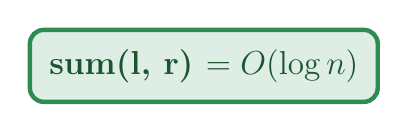
\begin{tikzpicture}
\node[draw=accentgreen, ultra thick, fill=softgreen, rounded corners=5pt, inner sep=7pt, font=\large\bfseries, text=accentgreen!60!black]
  {sum(l, r) $= O(\log n)$};
\end{tikzpicture}
\end{center}
}
\end{frame}

% % ---------------- SLIDE: MASTER'S THEOREM PROOF ----------------
% \begin{frame}{Why $O(q\log n)$? The Proof}
% \vspace{-0.1cm}
% \centering
% \small
% Each operation (one query or one update) touches $2$ subproblems of size $n/2$, plus $O(1)$ work to merge:
% \begin{center}
% \begin{tikzpicture}
% \node[draw=navy, thick, fill=lightblue!30, rounded corners=4pt, inner sep=7pt, font=\normalsize]
%   {$T(n) = 2\,T\!\left(\dfrac{n}{2}\right) + O(1)$};
% \end{tikzpicture}
% \end{center}
% \vspace{0.2cm}
% \onslide<2->{
% {\scriptsize Master Theorem: $a=2,\ b=2,\ f(n)=O(1)$ $\;\Rightarrow\;$ compare $n^{\log_b a}=n^1$ vs.\ $f(n)$ --- \textbf{$n^{\log_b a}$ dominates} $\Rightarrow$ Case 1.}
% \vspace{0.15cm}
% \begin{center}
% \begin{tikzpicture}
% \node[draw=accentgreen, thick, fill=softgreen, rounded corners=4pt, inner sep=7pt, font=\normalsize\bfseries, text=accentgreen!60!black]
%   {$T(n) = O(\log n)$ \normalfont{per operation}};
% \end{tikzpicture}
% \end{center}
% }
% \onslide<3->{
% \vspace{0.2cm}
% {\scriptsize Now run this $q$ times --- $q$ queries, $q$ updates, any mix:}
% \vspace{0.1cm}
% \begin{center}
% \begin{tikzpicture}
% \node[draw=gold, ultra thick, fill=gold!15, rounded corners=5pt, inner sep=8pt, font=\Large\bfseries, text=darkgold]
%   {Total time $= O(q \log n)$};
% \end{tikzpicture}
% \end{center}
% }
% \end{frame}


% ============================================================
% PART III -- TIME COMPLEXITY, LIMITS & REAL WORLD (Wasif)
% ============================================================
\setpresenter{Wasif --- Complexity, Extensions \& Applications}
\section{Part III --- Fast, Flexible, and Ready for the Real World}

% ---------------- SLIDE: BACK TO THE STOCK MARKET ----------------
\begin{frame}{Back to 9:31 AM}
\vspace{-0.1cm}
\centering
\small
Suppose our system tracks $n = 1024$ instruments and must process $q = 36$ billion operations (queries + updates combined) --- assuming $\sim$1 nanosecond per elementary step:
\vspace{0.25cm}

\begin{center}
\renewcommand{\arraystretch}{1.35}
\begin{tabular}{@{}lcc@{}}
\toprule
 & \textbf{Naive rescan} $O(qn)$ & \textbf{Segment tree} $O(q\log n)$ \\
\midrule
Raw ops & $36\times10^9 \times 1024$ & $36\times10^9 \times 10$ \\
\rowcolor{lightblue!30}
\textbf{Real time} & \textbf{$\approx 10.24$ hours} & \textbf{$= 6$ minutes} \\
\bottomrule
\end{tabular}
\end{center}
\vspace{0.35cm}

\onslide<2->{
\begin{center}
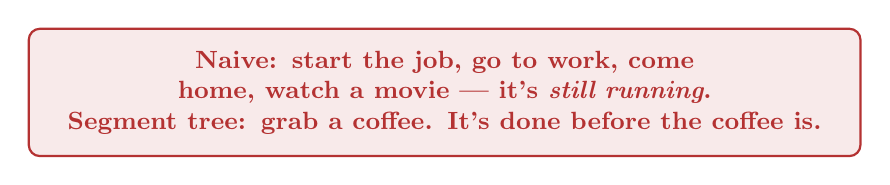
\begin{tikzpicture}
\node[draw=warningred, thick, fill=warningred!10, rounded corners=4pt, inner sep=8pt, font=\small\bfseries, text=warningred,
      text width=10cm, align=center]
  {Naive: start the job, go to work, come home, watch a movie --- it's \emph{still running}.\\
   Segment tree: grab a coffee. It's done before the coffee is.};
\end{tikzpicture}
\end{center}
}
\end{frame}

% ---------------- SLIDE 10: THE COMPLEXITY SHOWDOWN ----------------
\begin{frame}{The Complexity Showdown}
\vspace{-0.15cm}
\begin{center}
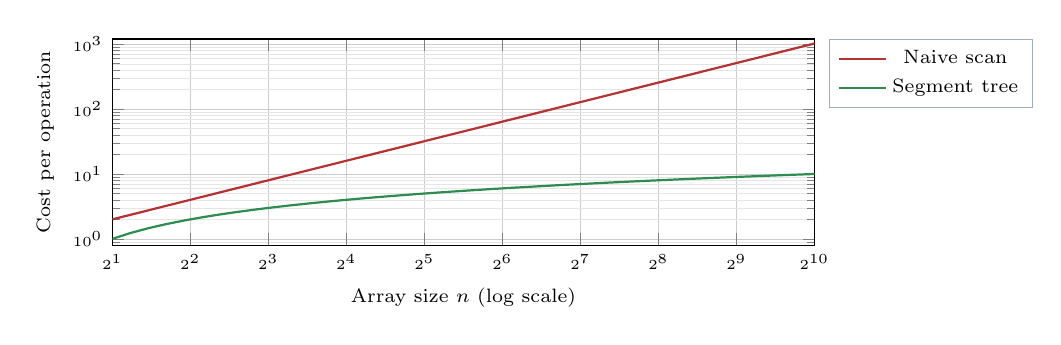
\begin{tikzpicture}
\begin{axis}[
  width=10.5cm, height=4.2cm,
  xlabel={Array size $n$ (log scale)},
  ylabel={Cost per operation},
  xmode=log, log basis x=2,
  ymode=log, log basis y=10,
  xmin=2, xmax=1024,
  ymin=0.8, ymax=1200,
  grid=both,
  major grid style={line width=.2pt, draw=gray!40},
  minor grid style={line width=.1pt, draw=gray!20},
  legend style={at={(1.02,1)}, anchor=north west, font=\scriptsize, draw=navy!40},
  every axis label/.append style={font=\scriptsize},
  tick label style={font=\tiny},
]
\addplot[thick, warningred, domain=2:1024, samples=40, mark=none] {x};
\addlegendentry{Naive scan}
\addplot[thick, accentgreen, domain=2:1024, samples=40, mark=none] {ln(x)/ln(2)};
\addlegendentry{Segment tree}
\end{axis}
\end{tikzpicture}
\end{center}
\vspace{0.15cm}
\small
\begin{center}
\renewcommand{\arraystretch}{1.2}
\begin{tabular}{@{}lccc@{}}
\toprule
\textbf{Structure} & \textbf{Query} & \textbf{Update} & \textbf{Build} \\
\midrule
Naive array          & $O(n)$      & $O(1)$      & --- \\
Prefix sums          & $O(1)$      & $O(n)$      & $O(n)$ \\
Fenwick tree         & $O(\log n)$ & $O(\log n)$ & $O(n\log n)$ \\
\rowcolor{lightblue!35}
\textbf{Segment tree} & $\boldsymbol{O(\log n)}$ & $\boldsymbol{O(\log n)}$ & $\boldsymbol{O(n)}$ \\
\bottomrule
\end{tabular}
\end{center}
\begin{center}
{\scriptsize\textcolor{accentgreen}{At $n=10^6$: naive $\approx 10^6$ ops/query --- segment tree $\approx 20$. That's the whole pitch.}}
\end{center}
\end{frame}

% ---------------- SLIDE: GENERALIZATION ----------------
\begin{frame}{Same Tree, Different Rules}
\small
\begin{center}
\renewcommand{\arraystretch}{1.3}
\begin{tabular}{@{}lll@{}}
\toprule
\textbf{Problem} & \textbf{Node stores} & \textbf{Combine rule} \\
\midrule
Range sum      & running total     & add \\
Range minimum  & smallest value    & take min \\
Range maximum  & largest value     & take max \\
Range GCD      & gcd so far        & gcd \\
\rowcolor{lightblue!30}
\textbf{...any associative rule} & \textbf{...any summary} & \textbf{...just swap it in} \\
\bottomrule
\end{tabular}
\end{center}
\vspace{0.3cm}
\begin{block}{Why this matters}
The \textbf{tree} never changes --- only what a node stores and how two nodes combine. Master one structure, unlock a dozen problems.
\end{block}
% ADDED: closing recap slide-within-slide, ties Part II together for the evaluator
\vspace{4pt}
{\centering\scriptsize\textcolor{navy!70}{\textbf{Recap --- Part II:} build once in $O(n)$, then update and query any range, with any associative rule, in $O(\log n)$ each.}}
\end{frame}

% ---------------- SLIDE 12: FROM SLIDES TO SERVERS ----------------
\begin{frame}{From Slides to Servers}
\small
\centering
Where does this actually run?
\vspace{0.2cm}

\begin{columns}[T]
\begin{column}{0.33\textwidth}
\centering
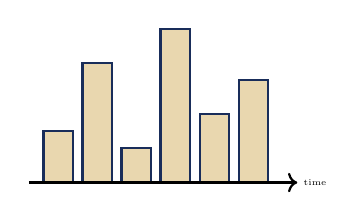
\begin{tikzpicture}[scale=0.62, every node/.style={transform shape}]
  \foreach \v [count=\i from 0] in {3,7,2,9,4,6}{
    \pgfmathsetmacro{\h}{\v*0.35}
    \draw[navy, thick, fill=gold!40] (\i*0.8,0) rectangle (\i*0.8+0.6,\h);
  }
  \draw[->, thick] (-0.3,0) -- (5.2,0) node[right, font=\tiny]{time};
\end{tikzpicture}
\\[2pt]
\textbf{Time-series \& stock feeds}\\
\scriptsize range-sum/min/max over any time window, instantly
\end{column}
\begin{column}{0.33\textwidth}
\centering
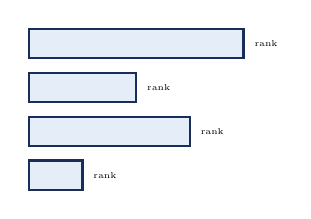
\begin{tikzpicture}[scale=0.62, every node/.style={transform shape}]
  \foreach \y [count=\i from 0] in {1,3,2,4}{
    \draw[navy, thick, fill=lightblue!50] (0,\i*0.9) rectangle (\y*1.1,\i*0.9+0.6);
    \node[font=\tiny, anchor=west] at (\y*1.1+0.1,\i*0.9+0.3) {rank};
  }
\end{tikzpicture}
\\[2pt]
\textbf{Live leaderboards}\\
\scriptsize $k$-th largest score \& rank updates in $O(\log n)$
\end{column}
\begin{column}{0.33\textwidth}
\centering
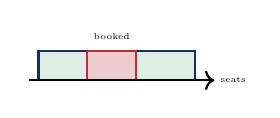
\begin{tikzpicture}[scale=0.62, every node/.style={transform shape}]
  \draw[navy, thick, fill=softgreen] (0,0) rectangle (3.2,0.6);
  \draw[warningred, thick, fill=warningred!25] (1.0,0) rectangle (2.0,0.6);
  \node[font=\tiny] at (1.5,0.9) {booked};
  \draw[->, thick] (-0.2,0) -- (3.6,0) node[right, font=\tiny]{seats};
\end{tikzpicture}
\\[2pt]
\textbf{Booking \& scheduling systems}\\
\scriptsize find/reserve a free range of seats or slots fast
\end{column}
\end{columns}
\vspace{0.3cm}
\begin{block}{The common thread}
Any system that needs \textbf{``summarize a range, then change part of it''} --- repeatedly, at scale --- is a segment tree in disguise.
\end{block}
\end{frame}

% ---------------- SLIDE 13: SEGMENT TREE VS FENWICK ----------------
\begin{frame}{Segment Tree vs Fenwick: Pick Your Fighter}
\centering
\begin{columns}[T]
\begin{column}{0.48\textwidth}
\centering
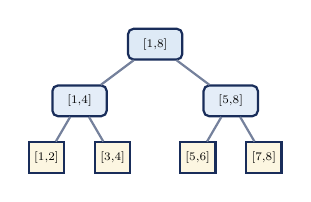
\begin{tikzpicture}[scale=0.6, every node/.style={transform shape}]
  \node[segnode, fill=lightblue!60] (r) at (0,0) {[1,8]};
  \node[segnode] (l) at (-1.6,-1.2) {[1,4]};
  \node[segnode] (rr) at (1.6,-1.2) {[5,8]};
  \node[segleaf] (a) at (-2.3,-2.4) {\scriptsize [1,2]};
  \node[segleaf] (b) at (-0.9,-2.4) {\scriptsize [3,4]};
  \node[segleaf] (c) at (0.9,-2.4) {\scriptsize [5,6]};
  \node[segleaf] (d) at (2.3,-2.4) {\scriptsize [7,8]};
  \draw[segedge] (r)--(l); \draw[segedge] (r)--(rr);
  \draw[segedge] (l)--(a); \draw[segedge] (l)--(b);
  \draw[segedge] (rr)--(c); \draw[segedge] (rr)--(d);
\end{tikzpicture}
\\[4pt]
\textbf{\large Segment Tree}
\end{column}
\begin{column}{0.48\textwidth}
\centering
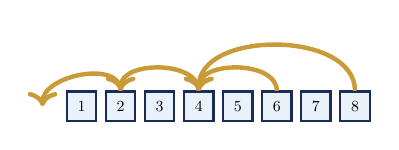
\begin{tikzpicture}[scale=0.62, every node/.style={transform shape}]
  \coordinate (f0) at (0,0);
  \foreach \i in {1,...,8}{
    \node[arrbox, minimum width=0.6cm, minimum height=0.6cm] (f\i) at (\i*0.8,0) {\i};
  }
  \draw[gold, ultra thick, ->] (f8) to[out=90,in=90] (f4);
  \draw[gold, ultra thick, ->] (f4) to[out=90,in=90] (f2);
  \draw[gold, ultra thick, ->] (f6) to[out=90,in=90] (f4);
  \draw[gold, ultra thick, ->] (f2) to[out=90,in=90] (f0.center);
\end{tikzpicture}
\\[4pt]
\textbf{\large Fenwick Tree (BIT)}
\end{column}
\end{columns}
\vspace{0.35cm}
\small
\renewcommand{\arraystretch}{1.25}
\begin{center}
\begin{tabular}{@{}lcc@{}}
\toprule
 & \textbf{Segment Tree} & \textbf{Fenwick Tree} \\
\midrule
Query / Update & $O(\log n)$ & $O(\log n)$ \\
Memory & $\sim 4n$ & $\sim n$ \\
Range updates (lazy) & \ding{51} natural & \ding{55} awkward \\
Flexibility (min/max/gcd/custom) & \ding{51} any associative op & \ding{55} sum-like only \\
Code footprint & larger & tiny \\
\bottomrule
\end{tabular}
\end{center}
\vspace{0.15cm}
{\scriptsize\textcolor{navy!70}{Fenwick wins on simplicity \& memory; segment tree wins on flexibility \& power. Pick based on what the problem demands.}}
\end{frame}

% ---------------- SLIDE 14: TAKEAWAYS + REFERENCES ----------------
\begin{frame}{Takeaways}
\small
\begin{columns}[T]
\begin{column}{0.55\textwidth}
\begin{itemize}\setlength{\itemsep}{6pt}
  \item[\textcolor{accentgreen}{\ding{51}}] Segment trees answer \textbf{range queries} and apply \textbf{updates}, both in $O(\log n)$.
  \item[\textcolor{accentgreen}{\ding{51}}] One structure, many rules: sum, min, max, gcd, or any associative merge.
  \item[\textcolor{accentgreen}{\ding{51}}] Powers real systems: finance, leaderboards, scheduling, and more.
\end{itemize}
\end{column}
\begin{column}{0.45\textwidth}
\centering
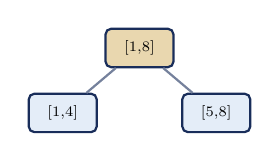
\begin{tikzpicture}[scale=0.75, every node/.style={transform shape}]
  \node[segnode, fill=gold!40] (r) at (0,0) {[1,8]};
  \node[segnode] (l) at (-1.3,-1.1) {[1,4]};
  \node[segnode] (rr) at (1.3,-1.1) {[5,8]};
  \draw[segedge] (r)--(l); \draw[segedge] (r)--(rr);
\end{tikzpicture}
\end{column}
\end{columns}
\vspace{0.3cm}
\begin{block}{References}
\scriptsize
CLRS, \textit{Introduction to Algorithms} --- Competitive Programmer's Handbook (Laaksonen) --- cp-algorithms.com, \textit{Segment Tree}
\end{block}
\end{frame}

\end{document}